\documentclass{beamer}

\usepackage[utf8x]{inputenc}
\usepackage{default}
\usepackage[slovene]{babel}

\title{Programiranje s KDE}
\author{Miha \v Can\v cula}

\begin{document}

\frame{\titlepage}

\begin{frame}{Za"cetek}
  \begin{block}{Potrebujemo}
    \begin{itemize}
      \item "Cas
      \item Angle"s"cino
      \item Osnovno znanje programiranja
      \item ``Srbenje''
    \end{itemize}
  \end{block}
  \begin{block}{Ne potrebujemo}
    \begin{itemize}
      \item O"cal, krivega nosu, hitrega tipkanja
      \item Iskanja blondink v padajo"cih zelenih znakih
      \item Novega hitrega ra"cunalnika
    \end{itemize}
  \end{block}
\end{frame}

\begin{frame}{S "cim za"ceti}
 \begin{columns}
  \begin{column}{.47\textwidth}
   \begin{block}{Nov program}
    \begin{itemize}
     \item Svobodna izbira programa 
     \item Prilagajanje lastnim "zeljam in potrebam \\[1cm]
     \item Motivacija, potrpe"zljivost
    \item Samostojno u"cenje in delo
    \end{itemize}
   \end{block}
  \end{column}
  \begin{column}{.47\textwidth}
   \begin{block}{Izbolj"sava obstoje"cega}
    \begin{itemize}
     \item Mo"znost pomo"ci s strani ostalih razvijalcev
     \item Preverjanje in potrditev
      \item Hitri rezultati \\[.5cm]
     \item Odvisnost od drugih
     \item Spoznavanje z obstoje"co kodo
    \end{itemize}
   \end{block}
  \end{column}
 \end{columns}
\end{frame}


\begin{frame}{Kompromisi}
\begin{block}{Mentorski programi}
\begin{itemize}
 \item Google Summer of Code -- pla"can
 \item Season of KDE -- prostovoljen
\end{itemize}
\end{block}
\begin{block}{Druge mo"znosti}
\begin{itemize}
 \item Vstavki z dolo"cenimi funkcijami (Kipi, Phonon, Cantor, KDevelop, ...)
 \item Kopiranje funkcionalnosti ne-KDE programov
 \item Vmesniki za programe z ukazne vrstice
\end{itemize}
\end{block}
\end{frame}

\begin{frame}{Pomo"c pri programiranju}
 \begin{itemize}
  \item TechBase -- wiki z navodili
  \item Mailing liste, IRC kanali, blogi
  \item Infrastruktura, shranjevanje kode, mo"znost pregleda prispevkov
  \item Preverjanje pogostih napak v kodi
  \item Razvojno okolje KDevelop
 \end{itemize}
\end{frame}

\begin{frame}{Knji"znice}
 \begin{block}{Uporabljene v Knights}
  \begin{itemize}
   \item KConfig
  \item Plasma -- namizje
  \item Solid -- strojna oprema
  \item KGameTheme, KGameRenderer
  \item KParts -- nalaganje delov programov
  \end{itemize}

 \end{block}
 \begin{block}{Ostale}
  \begin{itemize}
   \item Phonon -- ve"cpredstavnost
   \item Akonadi -- upravljanje z osebnimi podatki
  \item KIO -- omre"zni dostop
  \end{itemize}
 \end{block}
\end{frame}

\begin{frame}{KDevelop}
 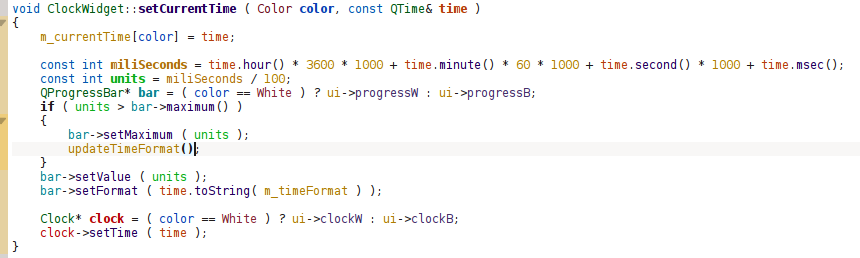
\includegraphics[width=\textwidth]{./KDE/kdev-color}
  \begin{itemize}
   \item Barve
   \item Samodejno dokon"cevanje
   \item Brskanje po dokumentaciji
  \end{itemize}
\end{frame}

\end{document}
